\newcounter{goals_counter}
\setcounter{goals_counter}{1}
\subsection{The Problem}
\begin{flushleft}
%%%%%%%%%%%%%%%%%%%%%%%%%%%%%%%%%%%
%%%%%%%%%%% THE PROBLEM %%%%%%%%%%%
%%%%%%%%%%%%%%%%%%%%%%%%%%%%%%%%%%%
The world's food supply chain is threatened by climate change and an unsustainable rate of rising population. Since the Telangana region largely participates in the world's food economy, the Telangana government is interested in pursuing initiatives aimed at mitigating the effect of these issues. More specifically, the Telangana government aims to reform the way they build their policies related to food production. Their goal is to utilize digital public goods and community-centric approaches in order to build resiliency against these dynamic challenges by building policies that are more agile and data-driven. 
\end{flushleft}
%%%%%%%%%%%%%%%%%%%%%%%%%%%%
%%%%%%%%% PURPOSE %%%%%%%%%%
%%%%%%%%%%%%%%%%%%%%%%%%%%%%
\subsection{Purpose}
\subsubsection{Purpose of the Document}
\begin{flushleft}
The purpose of this document is to present a comprehensive description of the requirements and specifications for the project. This document will specify all the information needed to understand exactly the requirements that should be satisfied. 
\end{flushleft} 

%%%%%%%%%%%%%%%%%%%%%%%%%%%%%%%%%%%
%%%%%% THE PROPOSED SOLUTION %%%%%%
%%%%%%%%%%%%%%%%%%%%%%%%%%%%%%%%%%%
\subsubsection{Purpose of the Product}
The purpose of the product is to provide a solution to address the problem previously outlined. 
This initiative, named {\bf D}ata-d{\bf R}iven Pr{\bf E}dictive F{\bf A}r{\bf M}ing, or DREAM, intends to provide a solution that focuses on serving the needs of three stakeholders: farmers, agronomists, and policy makers as shown in \textbf{Figure \ref{fig:stakeholders}}.


%%%%%%%%%%%%%%%%%%%%%%%%%%%%%%%%%%%
%%%%%%%%% GENERAL DIAGRAM %%%%%%%%%
%%%%%%%%%%%%%%%%%%%%%%%%%%%%%%%%%%%
\begin{figure}[hbt!]
\centering
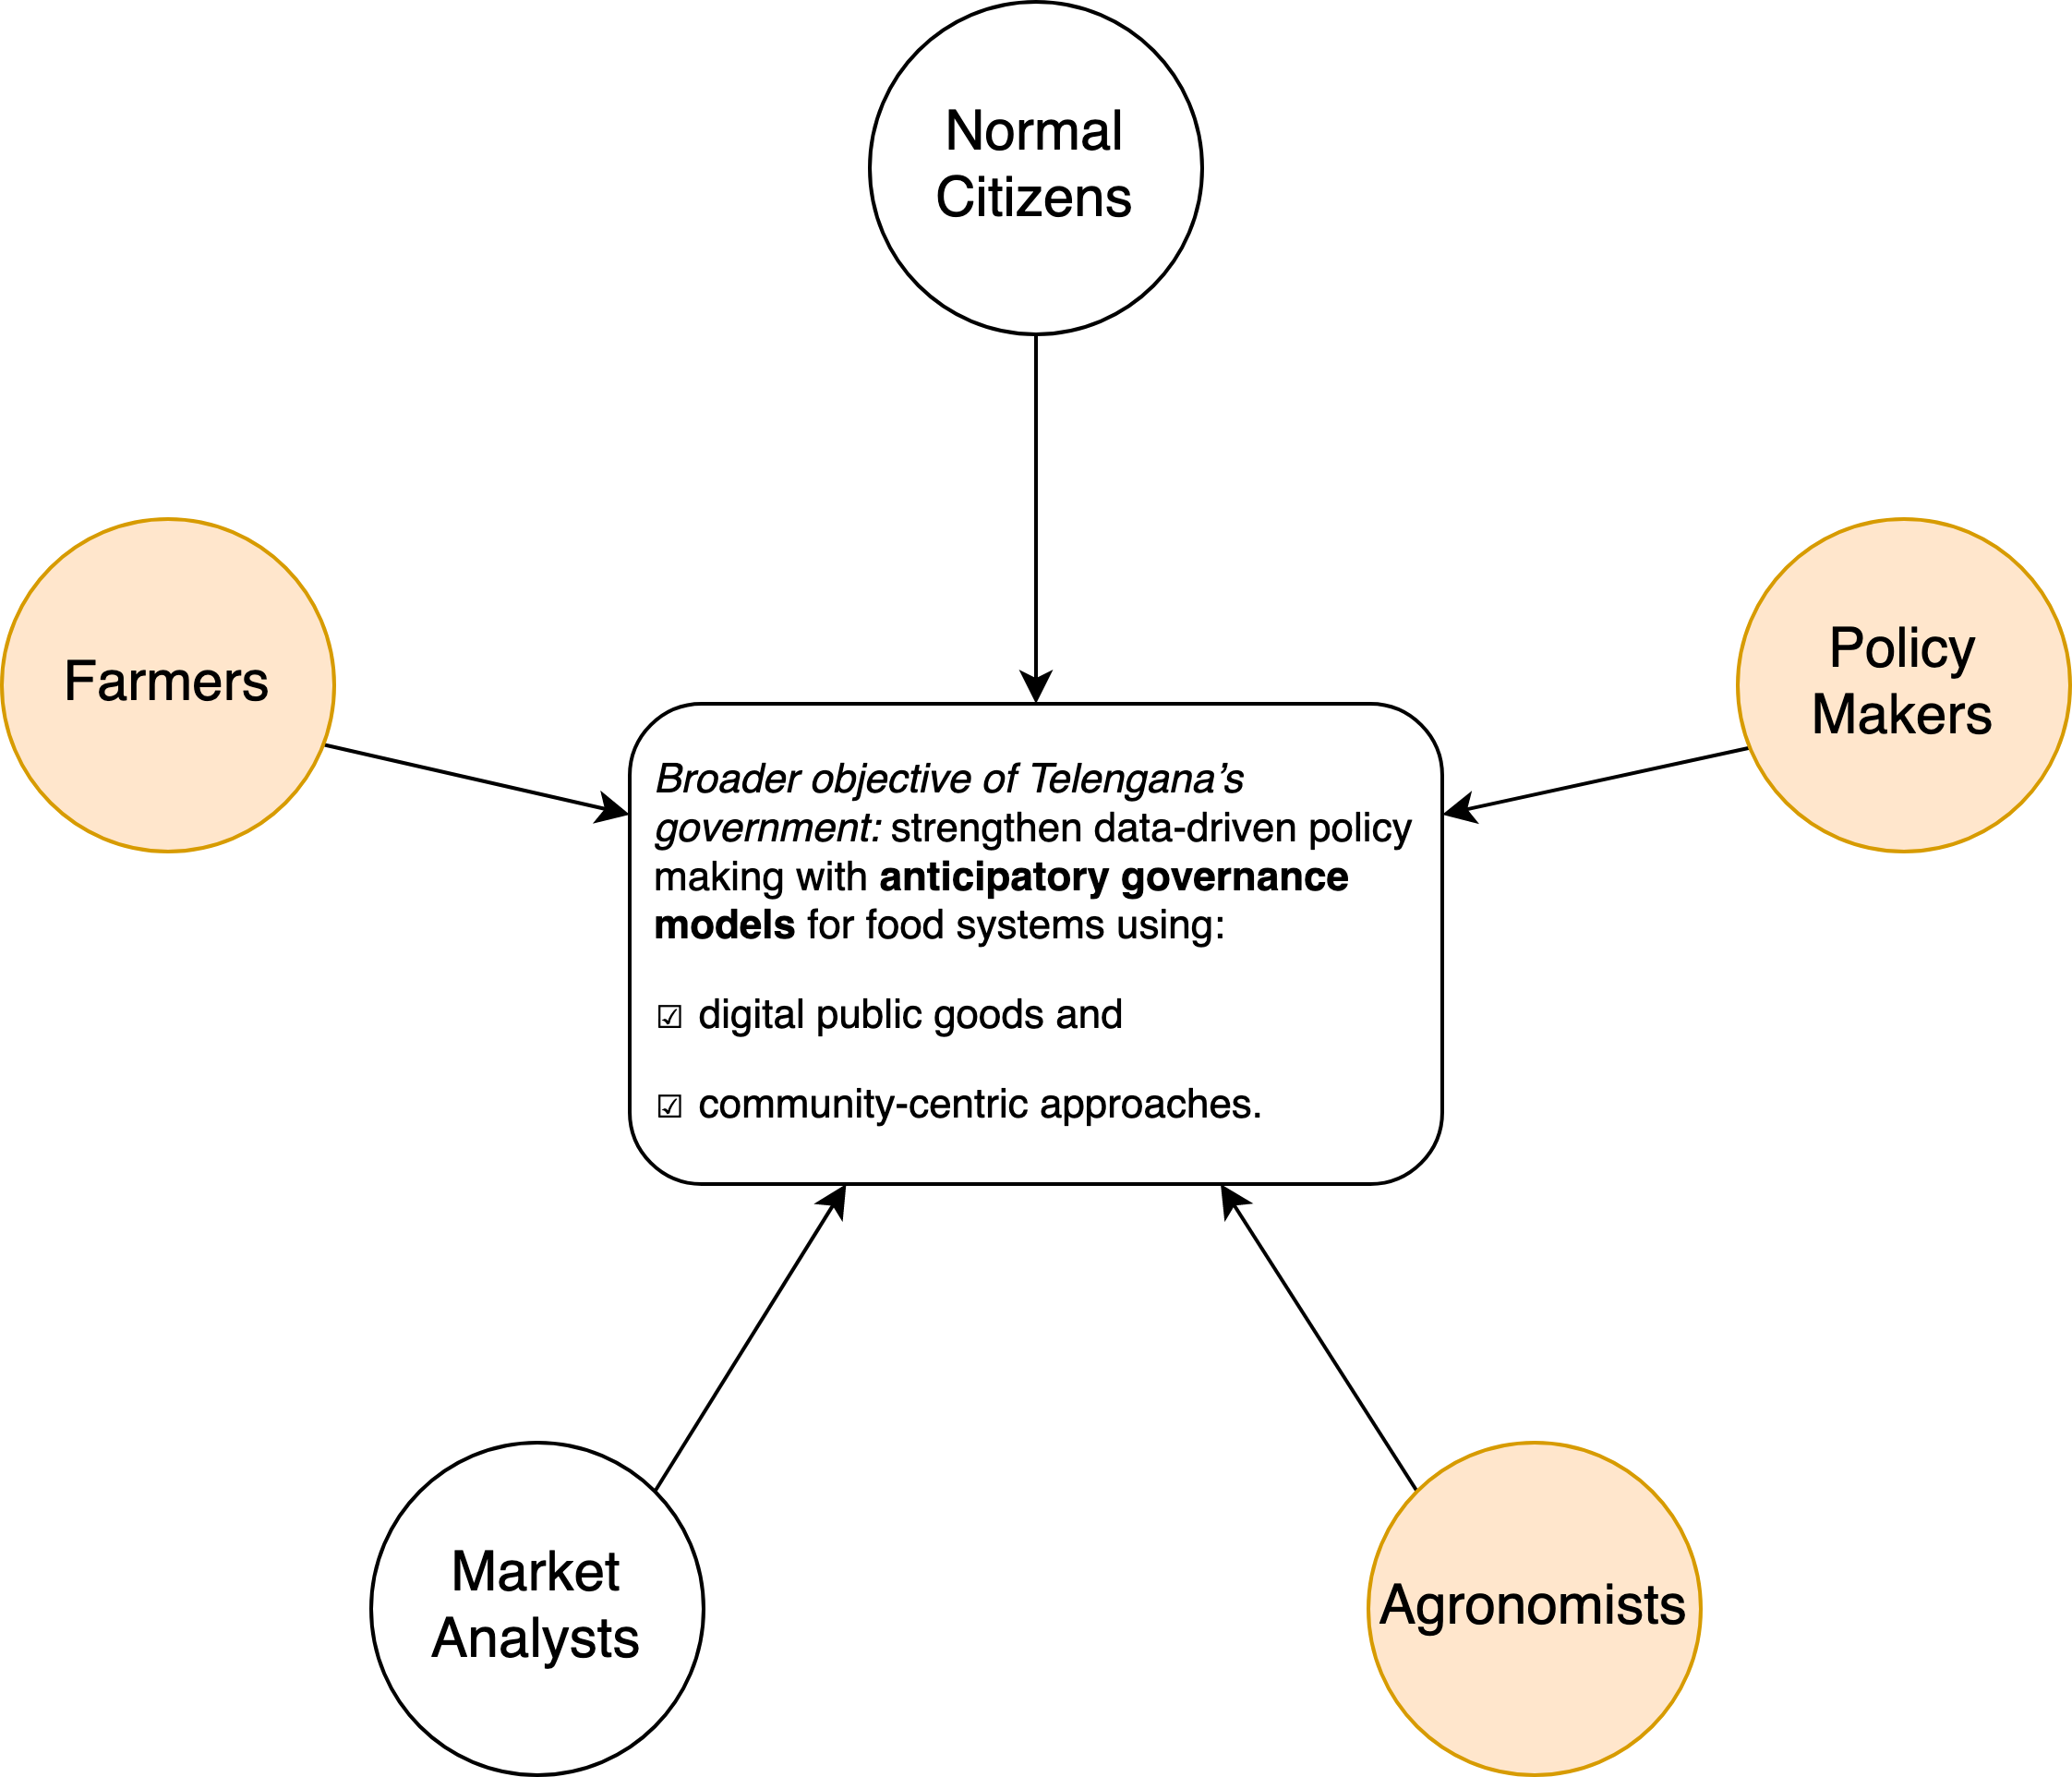
\includegraphics[scale=0.6]{../images_diagrams/stakeholders_in_broader_gov_objective.png}
\caption{Objective and stakeholders.}
\label{fig:stakeholders}
\end{figure}

\begin{flushleft}
The general aim is to take advantage of the present-day abundance of data and the potential for platforms to streamline communication. By utilizing data analysis, farmers can have access to automated solutions, therefore tackling their issues with agility and confidence. Additionally, by offering a means of communication, farmers can leverage their own community as a resource for information and support. Regarding policy makers and agronomists, the product will serve as a tool to aid their respective work-flows. 
\end{flushleft}

%%%%%%%%%%%%%%%%%%%%%%%%%%%%%%%%%%%
%%%%%%%%%%%% THE GOALS %%%%%%%%%%%%
%%%%%%%%%%%%%%%%%%%%%%%%%%%%%%%%%%%
\subsubsection{Goals} \label{goalsection}

The DREAM system is intended to provide a solution for the many issues that arise when the food production sector is strained by slow communication and ineffective policies. Regarding the utility for farmers, purpose of the DREAM system is to: serve as a tool for farmers to input and manage the data relevant to their farms, provide a discussion forum for farmers to draw support from their community, provide a messaging tool to make support from agronomists more accessible, provide farmers custom and automated suggestions from the raw data. For agronomists, the DREAM system serves as a tool to manage their work-flows such as: managing their responsible area, managing their daily plans, providing a messaging tool to easily communicate with farmers directly, and providing a visualization of the data regarding the farmers in their responsible area. Finally, DREAM serves policy makers by providing a tool to visualize the data and quantify the performance of the farmers from the entire Telangana region. \textbf{Table \ref{tab:goals}} provides an aggregate list of the specific goals that are to be accomplished by the DREAM system.

%%%% GOALS TABLE %%%%
\renewcommand{\arraystretch}{1.25}
\begin{table}[hbt!]
\centering
\small
\caption{\label{tab:goals}Goals of the system.}
\begin{tabular}{|c| >{\raggedright\arraybackslash}p{12cm}|} \hline
    \textbf{ID} & \textbf{Goals}\\
    \hline
    G\addOne{goals_counter}  & Farmers can visualize relevant data and suggestions based on their location and type of production.\\ 
    \hline
    G\addOne{goals_counter}  & Agronomists and farmers can view weather forecast data.\\ 
    \hline
    G\addOne{goals_counter}  & Farmers can interact with others farmers and agronomists by requesting for help and suggestions.\\
    \hline
    G\addOne{goals_counter}  & Farmers can create discussion forums with other farmers.\\
    \hline
    G\addOne{goals_counter}  & Agronomists can supervise a sub-area inside the region. \\
    \hline
    G\addOne{goals_counter}  & Agronomists can visualize the performance of the farmers in their sub-area.\\ %view the ranking of farmers’ performance in their specific area.
    \hline
    G\addOne{goals_counter}  & Agronomists can visualize and update a daily plan to visit farms in their area.\\
    \hline
    G\addOne{goals_counter}  & Agronomists can specify the deviations from their daily plan and confirm the execution of their daily plan at the end of each day.\\
    \hline
    G\addOne{goals_counter}  & Telengana’s policy makers can view the performance of the farmers and the ranking of the farmers.\\
    \hline
    G\addOne{goals_counter} & Telengana’s policy makers can determine if support from agronomists and well-performing farmers produces significant results.\\
    \hline
\end{tabular}
\end{table}


%%%%%%%%%%%%%%%%%%%%%%%%%%%%%%%%%%%
%%%%%%%%%%%%% PHENOMENA %%%%%%%%%%%
%%%%%%%%%%%%%%%%%%%%%%%%%%%%%%%%%%%

\subsection{Scope}

\begin{flushleft} 
Considering the three users in the scope of this initiative, farmers, agronomists, and policy makers, the design of the system must first consider the following phenomena to define the context in which the system will operate. 
% world phenomena description
The world phenomena specifies phenomena or attributes of the environment that merely exist. For example, WP2 in \textbf{Table \ref{tab:worldphenomena}} indicates that farmers will have issues on the farm, whether the system exists, or not.
% machine phenomena description
The machine phenomena specifies the phenomena that occur inside the system and because of the system. For example, MP5 in \textbf{Table \ref{tab:machinephenomena}} indicates that the best path connecting all the farmers in the daily plan will be calculated. This real-world event would not occur if the system did not exist. 
% shared phenomena description
The shared phenomena, however, specifies the phenomena that satisfy the descriptions for both the world and machine phenomena. For example, SP2 in \textbf{Table \ref{tab:sharedphenomena}} indicates that a farmer sends a message to the agronomist. This real-world event would still happen if the system did not exist, but due to the functionality offered by the DREAM product, this event occurs within the system. 
\end{flushleft}

%%%% PHENOMENA TABLE %%%%
\subsubsection{World Phenomena}
% the label is worldphenomena


\newcounter{phenomena_counter}
\setcounter{phenomena_counter}{1}
\begin{table}[hbt!]
\centering
\caption{\label{tab:worldphenomena} Phenomena related to the world.}
\renewcommand{\arraystretch}{1.25}
\begin{tabular}{|l|>{\raggedright\arraybackslash}m{12cm}|} \hline
    \textbf{World Phenomena} & \textbf{Description}\\\hline
	WP\addOne{phenomena_counter} & An agronomist visits a farm\\\hline
	WP\addOne{phenomena_counter} & Farmer has an issue with the farm\\\hline
\end{tabular}

\end{table}


\subsubsection{Shared Phenomena}
% the label is sharedphenomena
\newcounter{shared_counter}
\setcounter{shared_counter}{1}


\begin{table}[H]
\centering
\renewcommand{\arraystretch}{1.25}
%\begin{tabular}{|l|>{\raggedright\arraybackslash}m{12cm}|} \hline

\begin{tabular}{|m{3cm}|m{9cm}|m{3cm}|}
\hline
\textbf{Shared Phenomena}  & \textbf{Description} & \textbf{Who controls it} \\ \hline

SP\addOne{shared_counter} & An agronomist confirms a plan and send all the data about the visits he performed& W \\ \hline
SP\addOne{shared_counter} & A farmer sends a message to an agronomist &  W\\ \hline
SP\addOne{shared_counter} & A farmer creates a forum discussion  & W  \\ \hline
SP\addOne{shared_counter} & An agronomist responds to a farmer help or suggestion request  & W \\ \hline 
SP\addOne{shared_counter} & A user inspects data  & W \\ \hline
SP\addOne{shared_counter} & Policy maker flags poor performing and well performing farmers & W \\ \hline
\end{tabular}

\caption{World and Machine Phenomena table}
\label{PhenomenaTable}
\end{table}

\subsubsection{Machine Phenomena}
% the label is machinephenomena




\newcounter{machine_phenomena}
\setcounter{machine_phenomena}{1}

\begin{table}[hbt!]
\centering
\caption{\label{tab:machinephenomena} Phenomena related to the machine.}

\renewcommand{\arraystretch}{1.25}
\begin{tabular}{|l|>{\raggedright\arraybackslash}m{12cm}|} \hline
    \textbf{Machine Phenomena} & \textbf{Description}\\\hline
	MP\addOne{machine_phenomena} & An agronomist visits a farm\\\hline
	MP\addOne{machine_phenomena} & Farmer has an issue with the farm\\\hline
	MP\addOne{machine_phenomena} & Data analysis is performed \\ \hline
	MP\addOne{machine_phenomena} & Statistics are created based on data analyzed\\ \hline
	MP\addOne{machine_phenomena} & The system computes the best path connecting all farmers an agronomist has to visit \\ \hline
	MP\addOne{machine_phenomena} & The system recommend farmers to be visited by an agronomist\\ \hline

\end{tabular}
\end{table}

\subsection{Definitions, Acronyms, Abbreviations}

%%%% DEFINITIONS TABLE %%%%

\begin{center}
\renewcommand{\arraystretch}{1.25}
\begin{tabular}{l >{\raggedright\arraybackslash}p{12cm} } \hline
    \textbf{Term} & \textbf{Definition}\\ 
    DREAM & The system described in this document; Data-dRiven PrEdictive FArMing\\
    User & Farmer, agronomist, or policy user; anyone who uses the system.\\
	Policy Maker & Member of the Telangana government who deploys and manages different agriculture-related policies. \\
	Agronomist & Professional who specializes in agriculture sciences. \\
    Farmer & A user who uses DREAM to help manage data relating to their farms and fields.\\
    Field & One enclosed area that corresponds to one crop. Many fields can make up a farm. The locations of the various fields do not need to be co-located.\\
    Farm & A set of one or many fields that are managed by one farmer.\\
    Production yields & The amount of crop harvested compared to the amount of crop planted. Measured comparatively by percentage or numerically by weight.\\
    Flag & A marker on a farmer that signals the system to increase the priority for the farmer to get visited by an agronomist.\\
    TSDPS & Telangana State Development Planning Society which manages the automated weather stations around the state. \\
    World & A graphical representation of an instance of the Alloy model.\\
    UML & Unified Modeling Language\\
    MTTF & Mean Time To Failure\\
    MTTR & Mean Time To Recovery\\
    \hline
\end{tabular}
\end{center}

\subsection{Revision History}


\begin{flushleft}
\renewcommand{\arraystretch}{1.25}
\begin{tabular}{|c| l|>{\raggedright\arraybackslash}p{12cm} |} \hline
    \textbf{Revision} & \textbf{Date} & \textbf{Description}\\ \hline 
    1.0 & 20 December 2021 & Initial Release.\\
    \hline
\end{tabular}
\end{flushleft}


\subsection{Reference Documents}
\begin{itemize}
\item Assignment RDD A.Y. 2021-2022
\item \textit{Software Abstractions: Logic Language, and Analysis} by Daniel Jackson
\item ISO/IEC/IEEE 29148 dated 2018, Systems and software engineering - Life cycle processes - Requirements engineerings
\end{itemize}



\subsection{Document Structure}
The document is structured with the following sections:
\begin{itemize}
\item \textbf{Introduction}: This sections outlines the problem statement, the purpose of the document and of the project, the scope of the domain, and introduces the main goals of the system. 
\item \textbf{Overall Description}: This section goes into more detail about the main functions of the system. This description is aided with diagrams such as a class diagram for the system and flowcharts for select processes. The users of the system are also defined in this section. The system's domain is then described along with any dependencies and constraints. 
\item \textbf{Specific Requirements}: This section describes use cases further with a general use case diagram, use case tables, scenarios, and sequence diagrams. The individual requirements describing the entire system are listed and mapped to the goals and domain assumptions defined in the Introduction and in the Overall Description. Performance requirements and other design constraints are described at the end of the section.
\item \textbf{Formal Analysis Using Alloy}: The alloy code modeling the system is organized by general function. The facts are co-located with their associated signatures. The predicates and assertions are at the end of the code. Four different worlds have been generated, each one describing a different situation.
\item \textbf{Effort Spent}: For the purposes of the project assignment, this section itemized the time each participate allotted to different phases of the project. 
\item \textbf{References}: This section contains the bibliography for the document including all the relevant and cited documents.  
\end{itemize}


